\documentclass[twocolumn]{article}
\usepackage[top=1.1in, left=0.85in, right=0.85in]{geometry}

\usepackage{cite}
% \usepackage{eclbkbox}
\usepackage{amsmath}
\usepackage{amssymb}
% \usepackage{code}
% \usepackage{amscd}
% \usepackage{xy}
\usepackage{graphicx}
% \usepackage{fancyhdr}
% \usepackage{color}
% \usepackage[dark,all,bottom,landscape,timestamp]{draftcopy}
% \usepackage{everypage}

% \pagestyle{empty}

\usepackage{ulem}
% go back to italics for emphasis, though
\normalem

% \usepackage{inlinebib}

\newcommand\sfrac[2]{{}\,^{#1}\!/{}\!_{#2}}

\begin{document} 

\title{New results in $\sfrac{k}{n}$ Power-Hours}
\author{Dr.~Tom~Murphy~VII~Ph.D.\thanks{
Copyright \copyright\ 2014 the Regents of the Wikiplia
Foundation. Appears in SIGBOVIK 2014 with the chagrin of the
Association for Computational Heresy; {\em IEEEEEE!} press,
Verlag-Verlag volume no.~0x40-2A.
\yen 0.00}
}

\renewcommand\>{$>$}
\newcommand\<{$<$}
\newcommand\kn{\ensuremath{\sfrac{k}{n}\,}}

\newcommand\any{\ensuremath{\textrm{?}}}
\newcommand\nocup{\text{\sout{\ensuremath{\cup}}}}
\newcommand\fullcup{\ensuremath{\uplus}}
\newcommand\emptycup{\ensuremath{\cup}}
\newcommand\overcup{\ensuremath{\cap}}

\newcommand\nodrink{\ensuremath{\Rightarrow}}
\newcommand\drink{\ensuremath{\stackrel{{}^{\textrm{+}}}{\Rightarrow}}}

\date{1 April 2014}

\maketitle

\begin{abstract}
Something about the k-n hours

\end{abstract}

\vspace{1em}
{\noindent \small {\bf Keywords}:
  generalized binge drinking, maths,
  finite-state automata,
  abstract interpretation
}

\section*{Introduction}
A 2012 paper by Blum, Martens, Murphy, and Lovas\cite{algorithms}
introduced the \kn Power-Hour, a fractional variant on the well-known
drinking game. In a traditional Power-Hour, participants drink one
shot of beer per minute for 60 minutes. Since 5 beers in an hour
sometimes have adverse effects, some players opt for an attenuated
version of the game wherein fewer than 60 shots are consumed. However,
since the game is frantic and played simultaneous with others, it is
critical to have a mechanical procedure for performing the attenuated
Hour. The framework by Blum {\em et al.}, hereafter BMML, gives a
handful of simple operations that can be used to define a state
machine among $p$ players:
\begin{itemize}
  \item At the beginning of each minute, each player has at most one
    shot glass in front of him or her
  \item The shot glass must be in one of three states: Filled \fullcup,
    empty \emptycup, or overturned \overcup
  \item Atomically, each player performs an action based only on the
    state of his or her cup. If not in possession of a cup (written
    \nocup), the only action is to do nothing. With a cup:
  \begin{itemize}
    \item The player may drink \drink, or not drink \nodrink
    \item The player may pass the cup in any state to any player (a
      fixed player per action)
    \item However: If the cup is filled and the player did not drink,
      it must be passed in the filled state
    \item A player may not receive more than one cup in the same round
  \end{itemize}
\end{itemize}

Every assignment of rules and starting condition to $p$ players yields
a deterministic outcome, though some of these are illegal (because
they result in two or more cups being passed to the same player in
some round). For legal games, the outcome is that the $p$ players have
consumed $k_i$ shots of beer where $1 \leq i \leq p$ and $0 \leq k_i
\leq 60$. For the traditional power hour, the player starts with an
empty cup, at each step drinks,\!\footnote{In practice, this is done
  by filling the cup and then drinking it.} leaves the cup empty, and
passes to herself.

While the authors made a mostly clear definition of BMML and presented
some initial results, these results contained multiple serious errors
and the paper abruptly switches notation and assumptions several
times, and rambles incoherently. By their own admission, the authors
were drinking while they wrote it, taking only one hour to do so.
Don't drink and derive, kids!

This paper revisits the problem of BMML from a modern, sober
perspective, clarifies some of the original results, and presents
several new ones and a few conjectures.

\section{One-player \kn Power-Hours}

The goal of the \kn Power-Hour is to attenuate the number of drinks
consumed by the $p$ players, and its expressive power comes from the
ability to encode some state in the orientation of the cups, and
propagate that state via passing them from player to player. Even
without passing cups, the ability for a single player to attenuate his
drinking is nontrivial. Playing drinking games alone is sad indeed,
but the solo \kn Power-Hour still has practical applications. When
playing a Power Hour with others, if each player's desired $k$ is
attainable through solo methods then there is no need for passing
cups, which simplifies the ergonomics considerably. A common case is
where some of the players would like to do half--Power-Hours, which is
easily achieved in BMML by transitioning \emptycup\ to \fullcup\ without
drinking and \fullcup\ to \emptycup\ by drinking, and passing to
oneself.\!\footnote{There are many variations, but this was the
  strategy used many times in practice before being generalized to
  BMML.}

A full list of attainable \kn Power-Hours where $p=1$ appears in
Figure~\ref{fig:solo}. Possible values of $k$ are $\{ 0, 1, 2, 20, 29,
30, 31, 40, 58, 59, 60 \}$. The BMML paper claimed that the possible
values were $\{0, 1, 2, 20, 30, 40, 58, 59, 60 \}$, describing 31 for
example as ``super impossible.'' Achieving 31 is somewhat interesting.
One way to do it is to start with \emptycup, and use the rule that
\emptycup\ means drink and then fill the cup. We then use the rule
that \fullcup\ means drink and flip the cup, and \overcup\ means don't
drink and fill the cup. Essentially we use \emptycup\ to mean ``this
is the very first state'' and then take shots on alternating minutes
by using \overcup\ and \fullcup\ to encode the parity. Exploiting
non-steady-states like this (Figure~\ref{fig:solo31}) is how we
achieve $k$ that does not divide $n$.

\begin{figure}[ht]
\begin{center}
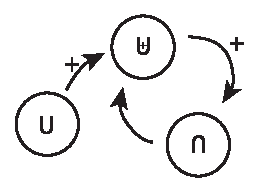
\includegraphics[width=0.90 \linewidth]{solo31.pdf}
\end{center}\vspace{-0.1in}
\caption{State machine that achieves $k=31$ in a solo BMML Power Hour.
  $+$ on an edge means the player drinks. The player always passes to
  herself.}
\label{fig:solo31}
\end{figure}

It is tractable to work out the possibilities for the solo case by
hand, though apparently not while drinking~\cite{algorithms}. These
results were generated by a computer program, which is probably
necessary for $p>1$. The next section describes how we explore this
space computationally.

\begin{figure}[ht]
\begin{center}
\begin{tabular}{c|ll}
$k$ & start & rules \\
\hline
0  &   \nocup    &  \emptycup \nodrink \any     , \overcup \nodrink \any      , \fullcup \nodrink \any \\
1  &   \emptycup &  \emptycup \drink \overcup   , \overcup \nodrink \overcup  , \fullcup \nodrink \any \\
2  &   \emptycup &  \emptycup \drink \fullcup   , \overcup \nodrink \overcup  , \fullcup \drink \overcup \\
20 &   \emptycup &  \emptycup \nodrink \overcup , \overcup \nodrink \fullcup  , \fullcup \drink \emptycup \\
29 &   \emptycup &  \emptycup \nodrink \overcup , \overcup \nodrink \fullcup  , \fullcup \drink \overcup \\
30 &   \emptycup &  \emptycup \drink \overcup   , \overcup \nodrink \emptycup , \fullcup \nodrink \any \\
31 &   \emptycup &  \emptycup \drink \fullcup   , \overcup \nodrink \fullcup  , \fullcup \drink \overcup \\
40 &   \emptycup &  \emptycup \drink \overcup   , \overcup \nodrink \fullcup  , \fullcup \drink \emptycup \\
58 &   \emptycup &  \emptycup \nodrink \overcup , \overcup \nodrink \fullcup  , \fullcup \drink \fullcup \\
59 &   \emptycup &  \emptycup \nodrink \overcup , \overcup \drink \overcup    , \fullcup \nodrink \any \\
60 &   \emptycup &  \emptycup \drink \emptycup  , \overcup \nodrink \any      , \fullcup \nodrink \any \\
\end{tabular}
\end{center}
\label{fig:solo}
\caption{All the possible $k$ for a solo Power-Hour in BMML. A
  superscript $+$ means that the player drinks. The symbol \any\ means
  that any cup state can be used in that position. Note that 29 and 58
  require wasting a shot of beer; all the others but 31 permit a
  variant where a shot is wasted as well.}
\end{figure}

\section{Two-player \kn Power-Hours}

For two players, it is easy to see how one of them could 

\begin{figure}
\begin{center}

\includegraphics[width=0.90 \linewidth]{3and2.pdf}
\end{center}\vspace{-0.1in}
\caption{Outcomes possible for the first two players in all different
  3-player power hours (black), overlayed by all possible outcomes
  outcomes for 2-player power hours (red). Mainly included because
  it looks pretty sweet.
}
\label{fig:3and2}
\end{figure}

\begin{figure}
\begin{center}
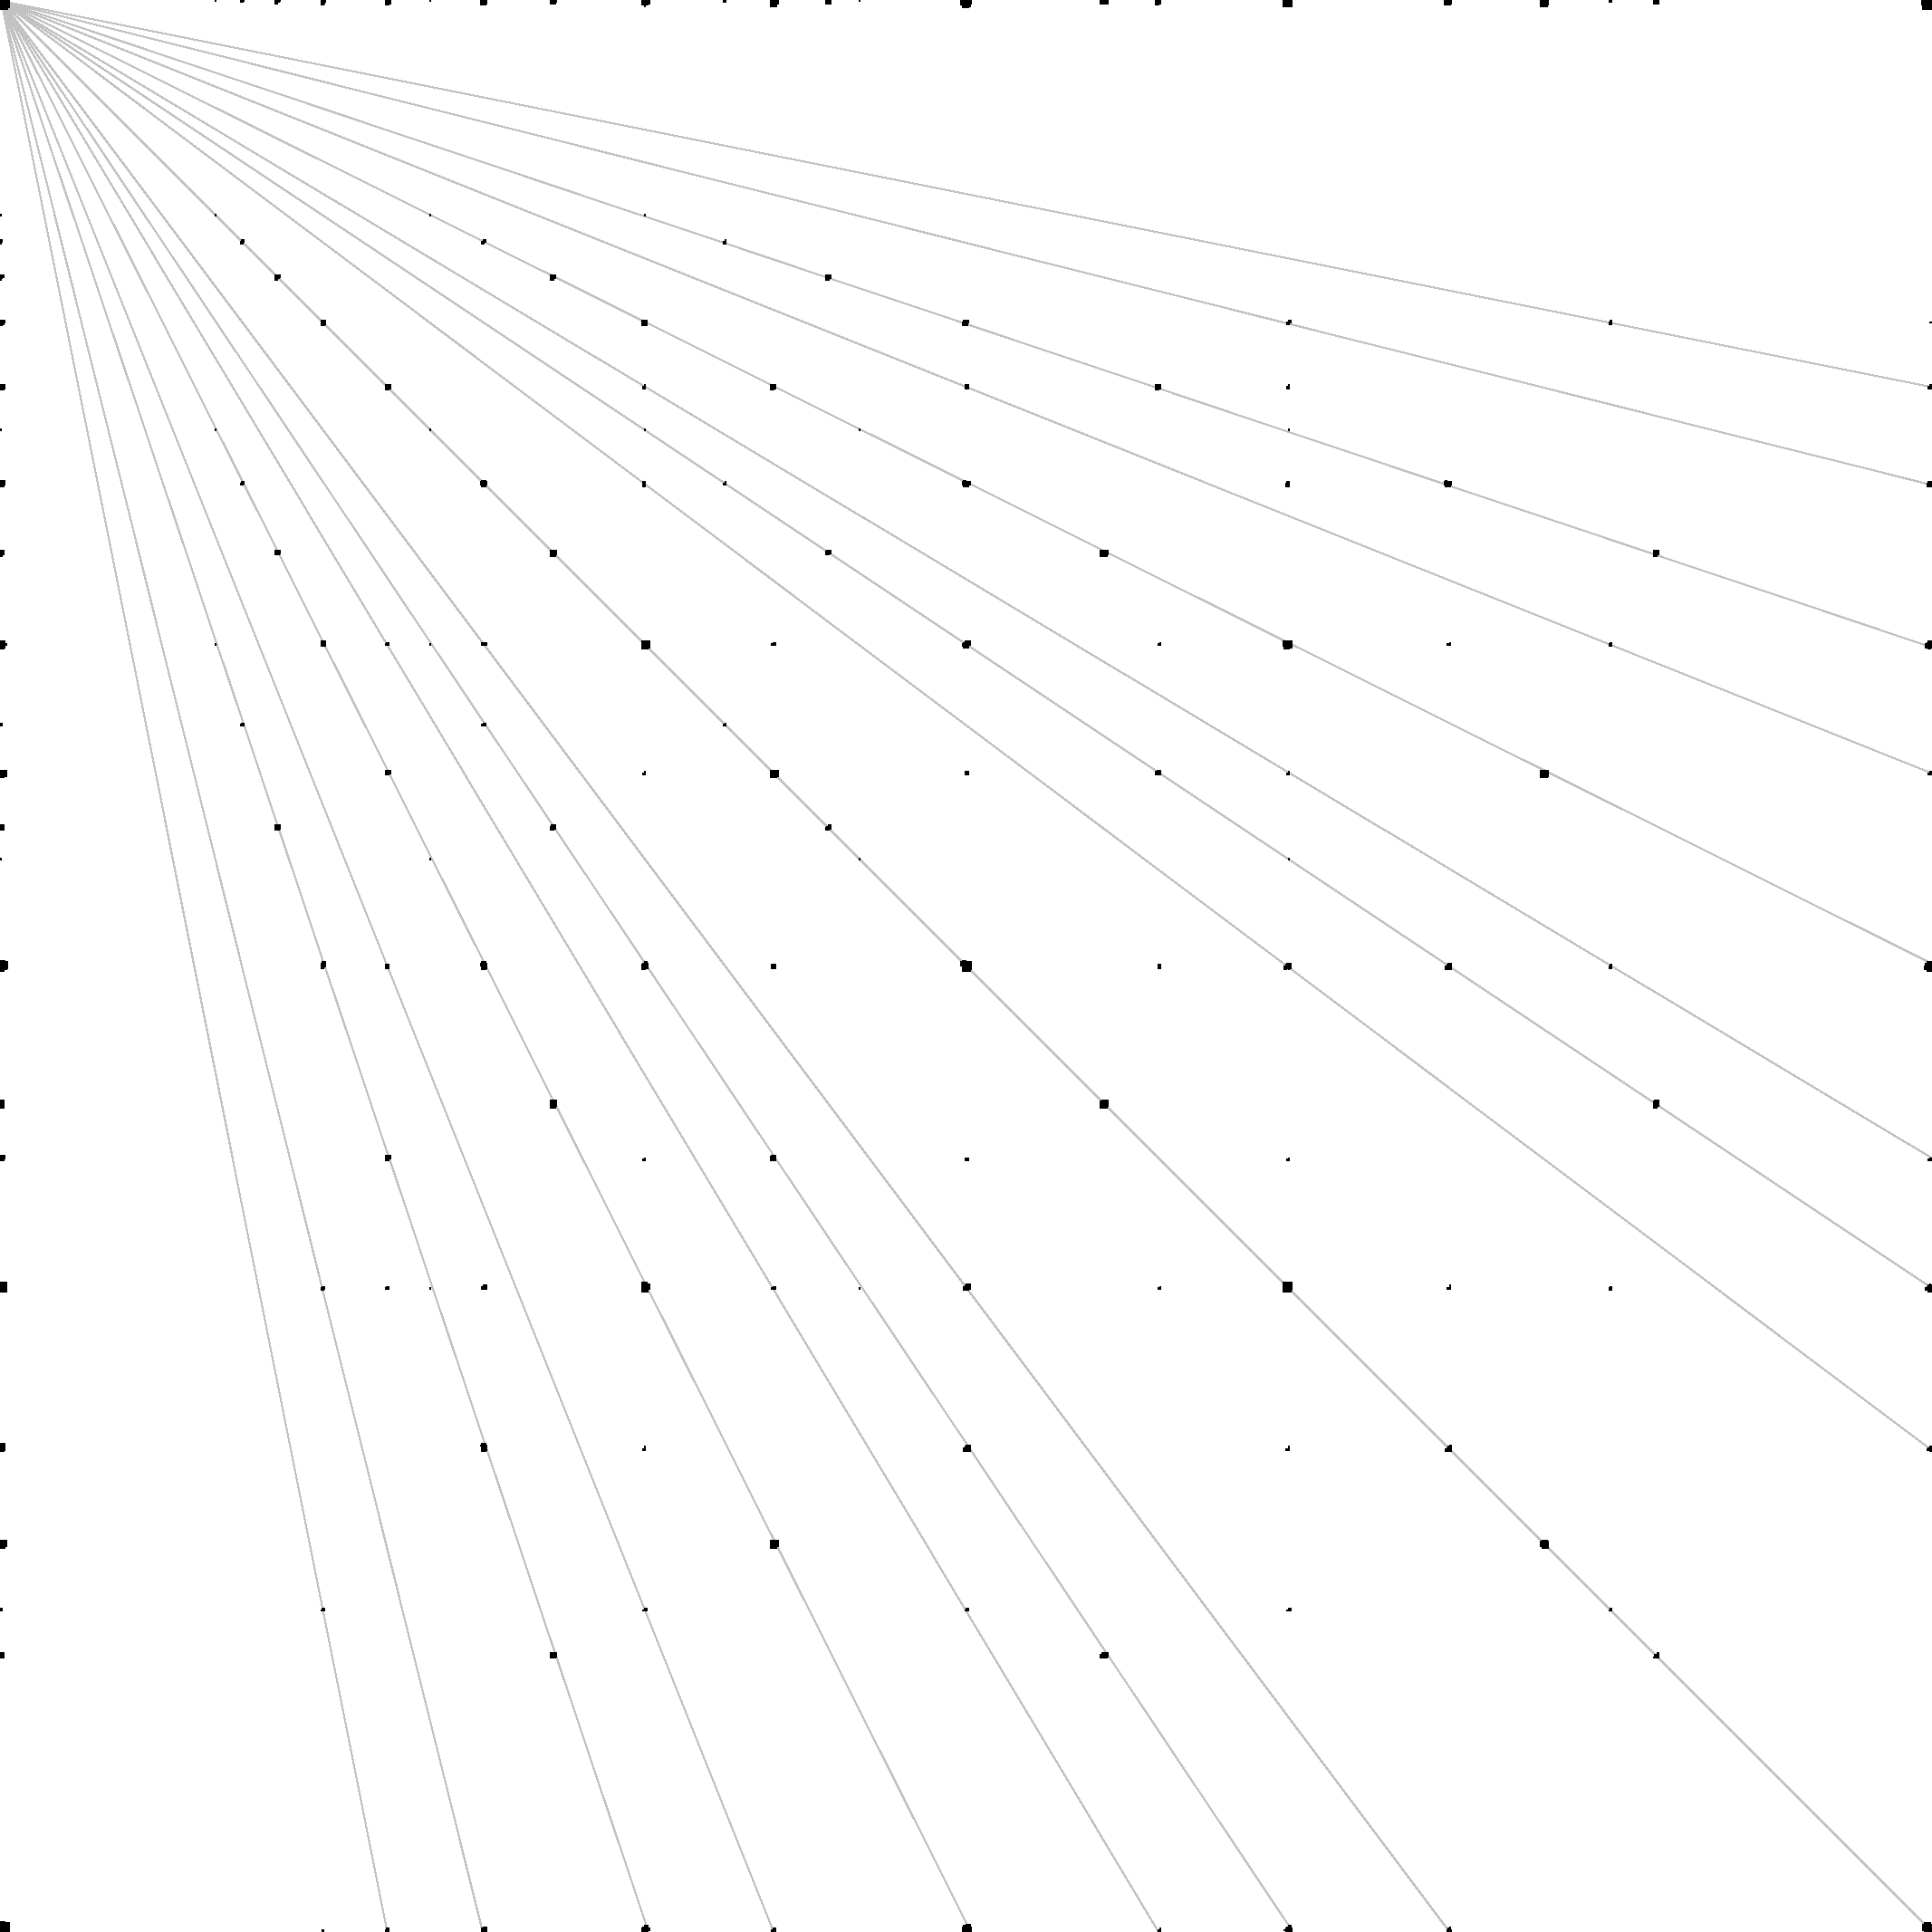
\includegraphics[width=0.90 \linewidth]{powerday3.pdf}
\end{center}\vspace{-0.1in}
\caption{All possible outcomes for the first two players in 3-player
  power days. These are the same games as the 3-player power hours,
  but at this scale makes it clear the groupings and their sparsity
  in the limit. Lines plotted from (0,0) to (60,*) and (*,60) show
  significant structure, but don't explain some of the interior points.
  (TODO: what are these games? what did the other player drink?)
}
\label{fig:powerday3}
\end{figure}

\section{Some stuffff}

Hi



\bibliography{paper}{}
\bibliographystyle{plain}
\end{document}
